\section{Circle Geometry}

A circle with centre at a point \(O\) and with radius \(r\) will be denoted \(\mathcal{C}(O, r)\).

\subsection{Inversion}

\begin{theorem}
    For circle \(\mathcal{C}(O, r)\), let \(P \neq O\) be any point and \(X, Y\) the intersection of \(\mathcal{C}\) and the line through \(O\) and \(P\) as below. Then \((X, Y; P, P') = -1\) if and only if \(OP \cdot OP' = r^2\).

    \begin{center}
        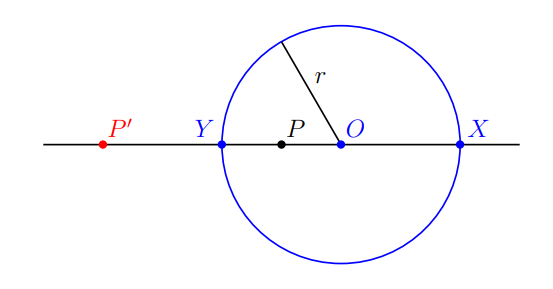
\includegraphics{assets/circle/inversion.png}
    \end{center}
\end{theorem}

\defn{Inverse}{
    Let \(\mathcal{C}(O, r)\) be a circle. Given a point \(P\) distinct from \(O\) we can define a point \(P'\) called its inverse in \(\mathcal{C}\) as follows: on the line \(OP\) the point \(P'\) is such that \(OP \cdot OP' = r^2\).
}

\begin{definition}
    The map \(T: \bR^2 \setminus \{0\} \to \bR^2 \setminus \{0\}\) sending each \(P\) to its inverse in \(\mathcal{C}\) is called inversion. We call \(O\) the centre of inversion and \(r\) the radius of inversion.
\end{definition}

Simple properties of an inversion, \(T\), are immediate:
\begin{itemize}
    \item \(T\) pointwise fixes the circle (if \(P\) is on the circle \(T(P) = P\));
    \item \(T\) maps the inside of the circle to the outside and vice versa;
    \item \(T\) is an involution, that is \(T^2(P) = P\).
\end{itemize}

\begin{theorem}
    If a circle \(\mathcal{C}(O, r)\) inverts \(A, B\) to \(A', B'\) respectively, then
    \[A'B' = \frac{r^2 AB}{OA \cdot OB}.\]
\end{theorem}

\begin{theorem}
    Let \(A, B, C, D\) be 4 points all distinct from \(O\). If circle \(\mathcal{C}(O, r)\) inverts \(A, B, C, D\) to \(A', B', C', D'\) respectively, then
    \[(A, B; C, D) = (A', B'; C', D').\]
\end{theorem}

\subsection{Poles and Polar}

\defn{Polar and Poles}{
    \setlength{\parindent}{1em}
    Let \(\mathcal{C}(O, r)\) be a circle. For a point \(P \neq O\) its polar, \(p\), is the line through its inverse point \(P'\) orthogonal to \(OP'\).

    Conversely, given a line \(\ell\) not through \(O\) its pole, \(L\), is the inverse point to the point \(L'\) closest to \(O\).
}

\begin{theorem}
    If \(P\) is external to \(\mathcal{C}(O, r)\), then its polar, \(p\), is the line through the points where the tangents from \(P\)meet the circle.
\end{theorem}

\begin{corollary}
    There is a ruler and compass construction of the tangents to a circle from an arbitrary external point.
\end{corollary}

\begin{theorem}
    \setlength{\parindent}{1em}
    For \(\mathcal{C}(O, r)\) and a point \(P\) that is neither \(O\) nor a point on the circle, suppose a line \(\ell\) through \(P\) intersects \(\mathcal{C}\) at distinct points \(X\) and \(Y\).

    Then if \(E\) is the intersection of \(\ell\) and the polar of \(P, \ell\)is divided harmonically by \(X, Y, E\) and \(P\): i.e. \((X, Y; E, P) = -1\).

    Conversely, if \(E\) on \(\ell\) is such that \((X, Y; E, P) = -1\), then the line perpendicular to \(OP\) through \(E\) is the polar of \(P\).
\end{theorem}

\begin{theorem}
    \setlength{\parindent}{1em}
    Let \(\mathcal{C}(O, r)\) be a circle. If \(\ell\) is any line not passing through \(O\), its inverse is a circle through \(O\) (minus the point \(O\)).

    Conversely, if \(\mathcal{C}'\) is a circle through \(O\), its inverse is a line perpendicular to the diameter of \(\mathcal{C}'\) through \(O\).
\end{theorem}

\begin{corollary}
    A circle \(\mathcal{C}'\) passing through \(O\) is inverted in circle \(\mathcal{C}(O, r)\) to a line parallel to the tangent to \(\mathcal{C}'\) at \(O\).
\end{corollary}

\begin{theorem}
    \setlength{\parindent}{1em}
    For \(\mathcal{C}(O, r)\) and \(L \neq O\), let \(\ell\) be its polar. Then for any point \(Q\) on \(\ell\), the polar of \(Q, q\), passes through \(L\).

    Conversely, for \(\ell\) a line not passing through \(O\) with pole \(L\), any line \(q\) through \(L\) has pole \(Q\) on \(\ell\).
\end{theorem}

\begin{corollary}
    For given circle \(\mathcal{C}(O, r)\), let \((P, p)\) and \((Q, q)\) be two pole/polar pairs, where \(N = p \cap q\) exists. Then the line \(PQ\) is the polar, \(n\), of \(N\) and the pole of \(PQ\) is \(N\).
\end{corollary}

\subsection{Intersection of Circles}

In general, two curves intersecting at a point \(P\) are said to be \textbf{orthogonal} if their tangents at \(P\) are orthogonal.

\begin{theorem}
    Two intersecting circles are orthogonal if and only if the angles in opposite segments are complementary.
\end{theorem}

\begin{theorem}
    \setlength{\parindent}{1em}
    Let \(A, B, C, D\) be a harmonic set, \((A, B; C, D) = -1\). The two circles with diameters \(AB\) and \(CD\) are orthogonal.

    Conversely, if two circles with centres \(O_1\) and \(O_2\) are orthogonal, and the line \(O_1O_2\) intersects one circle at \(A\) and \(B\) and the other at \(C\) and \(D\) then \((A, B; C, D) = -1\).
\end{theorem}

\subsection{Inverting Circles and Lines}

Given a circle \(\mathcal{C}(O, r)\), we saw in a previous result t hat a circle through \(O\) is inverted to a line not through \(O\), and conversely. It is clear that a line through \(O\) is inverted to a line through \(O\), namely the same line.

\begin{theorem}
    Let \(\mathcal{C}(O, r)\) be a circle and \(\Sigma(\Omega, \rho)\) a second circle not passing through \(O\). Under inversion in \(\mathcal{C}\), \(\Sigma\) is inverted to another circle not through \(O\).
\end{theorem}

\begin{theorem}
    Let \(\mathcal{C}(O, r)\) be a circle and \(\Sigma(\Omega, \rho)\) a second circle meeting \(\mathcal{C}\) orthogonally. Then \(\Sigma\) is inverted to itself in \(\mathcal{C}\).
\end{theorem}

When inverting in a circle \(\mathcal{C}(O, r)\), we avoided inverting \(O\) itself. However, we can imagine adding a \textbf{ideal point}, \(\infty\) ``at infinity'' to the plane, to which \(O\) is mapped by inversion in a circle centred at \(O\). \\

This extended plane has many nice properties, which will explore later, but here we note that we can think of a line in the plane as a circle through \(\infty\) in the extended plane. Then we can sum up our results on inversion as:

\begin{theorem}
    In the extended plane, inversion in a fixed circle maps a circle to a circle.
\end{theorem}

Clearly any translation or rotation about a fixed point will send a line to a line and a circle to a circle. It follows that the most general transformation that maps a circle or line to a circle or line is in fact a composition for a translation, a rotation and an inversion. \\

Thinking of \(\bR^2\) as \(\bC\), inversion in the circle \(|z - c| = r\) is the map \(z \mapsto c + \frac{r^2}{|z - c|^2}(z - c)\) and is the composition of conjugation and a special case of a \textbf{linear fractional transformation},
\[z \mapsto \frac{az + b}{cz + d}.\]